\documentclass[a4paper,titlepage]{article}
\title{Zelflerende Systemen}
\author{Steven Bronsveld en Thijs van Loenhout}

\usepackage[dutch]{babel}
\usepackage{graphicx}
\usepackage{multirow}
\usepackage{blindtext}
\usepackage{csquotes}
\usepackage{float}
\usepackage{amsmath}
\usepackage[backend=bibtex,sorting=none]{biblatex}
\usepackage{color}

\bibliography{references.bib}

\definecolor{praktijk}{rgb}{1,0.5,0}

\MakeOuterQuote{"}

\graphicspath{ {res/} }

\begin{document}

\textcolor{praktijk}{
	\section{Praktijk II: Neural network}
}


\subsection{Inleiding}
Met de kennis die we hebben opgedaan bij het maken van het theorieverslag gaan we zelf een praktijkopdracht uitvoeren. We dagen onszelf uit tot het zelf maken van een computerprogramma dat de volgende vraag beantwoordt: \textit{welke onderdelen zijn nodig voor een zelflerend computersysteem, in de vorm van een door ons ontworpen computerprogramma, dat in staat is afbeeldingen te classificeren binnen vastgestelde categorie\"en met een precisie van meer dan 80 procent?}

\subsection{Werkwijze}
Voordat we kunnen beginnen aan het ontwerp van het systeem moeten we eerst duidelijk maken wat we precies willen bereiken en hoe we dat willen bereiken. We moesten een aantal vragen eerst beantwoorden:\\
\textbf{Welke afbeeldingen gaan we proberen te classificeren?}\\
We gaan proberen handgeschreven cijfers te classificeren. We gebruiken hiervoor de MNIST dataset. [TODO] Dit is een dataset van een groot aantal afbeeldingen van handgeschreven cijfers met het bijbehorende label. De afbeeldingen zijn elk 28 x 28 pixels groot. Deze dataset is erg geschikt om Machine Learning op toe te passen.\\
\textbf{Welk algoritme gebruiken we voor het classificeren van de afbeeldingen?}\\
Wij gebruiken een Neural Network (TODO) om deze afbeeldingen te classificeren. Het is gebleken dat dit het beste algoritme is voor het classificeren van afbeeldingen. Er zijn 28 * 28 = 784 input neuronen en 10 output neuronen. We kiezen ervoor om één hidden layer te maken.\\
\textbf{Welke manier van leren gebruiken we voor het verbeteren voor het algoritme?}\\
We gaan gebruik maken van Gradient Descent (TODO). Dit lijkt ons de meest geschikte leer strategie voor dit probleem.

\subsection{Netwerk}
Het aantal input neuronen en het aantal output neuronen staat vast (respectievelijk 784 en 10). Het aantal hidden neuronen kunnen we zelf bepalen. Ook moeten nog aan elke laag een bias toevoegen (TODO). Zoals uitgelegd in (TODO) moeten we ook een \textit{activation function} kiezen. Hiervoor gebruiken we een sigmoid functie (zie figuur \ref{fig:sigmoid-function}). De lagen zijn onderling volledig verbonden. Elke verbinding heeft zijn eigen weging die op het begin naar een willekeurige waarde wordt gezet.

\begin{figure}[H]
	\begin{align*}
	   f(x) = \frac{1}{1 + e^{-u}}
	\end{align*}
	\caption{De sigmoid functie}
\end{figure}

\begin{figure}[H]
  \centering
    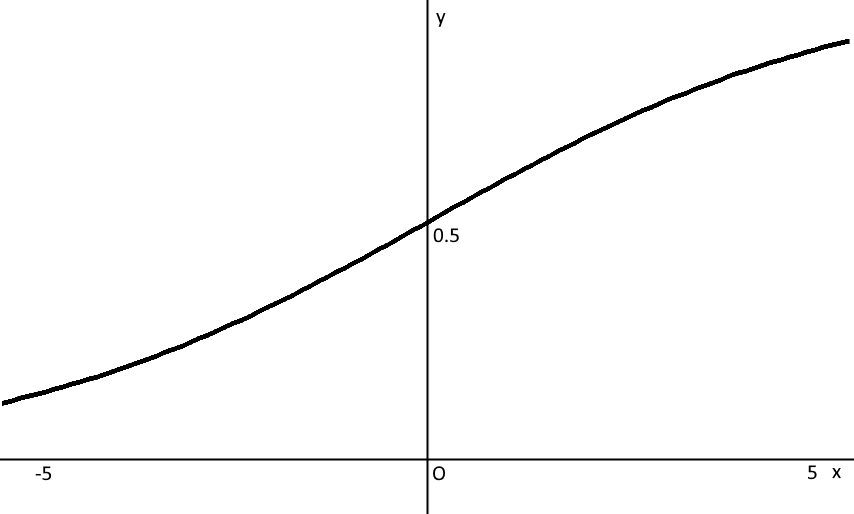
\includegraphics[width=0.5\textwidth]{sigmoid.png}
  \caption{De grafiek van de sigmoid functie}
  \label{fig:sigmoid-function}
\end{figure}


\subsection{Gradient descent}
Nu we een werkend netwerk hebben kunnen we naar het belangrijkste deel kijken: het vinden van de juiste wegingen voor de neuronen. Zoals gezegd gaan we dit doen door middel van gradient descent.
Wat we gaan doen is: \textit{het bepalen van de afgeleide van de cost function relatief tot de te veranderen variable.}

\begin{figure}[H]
  \centering
    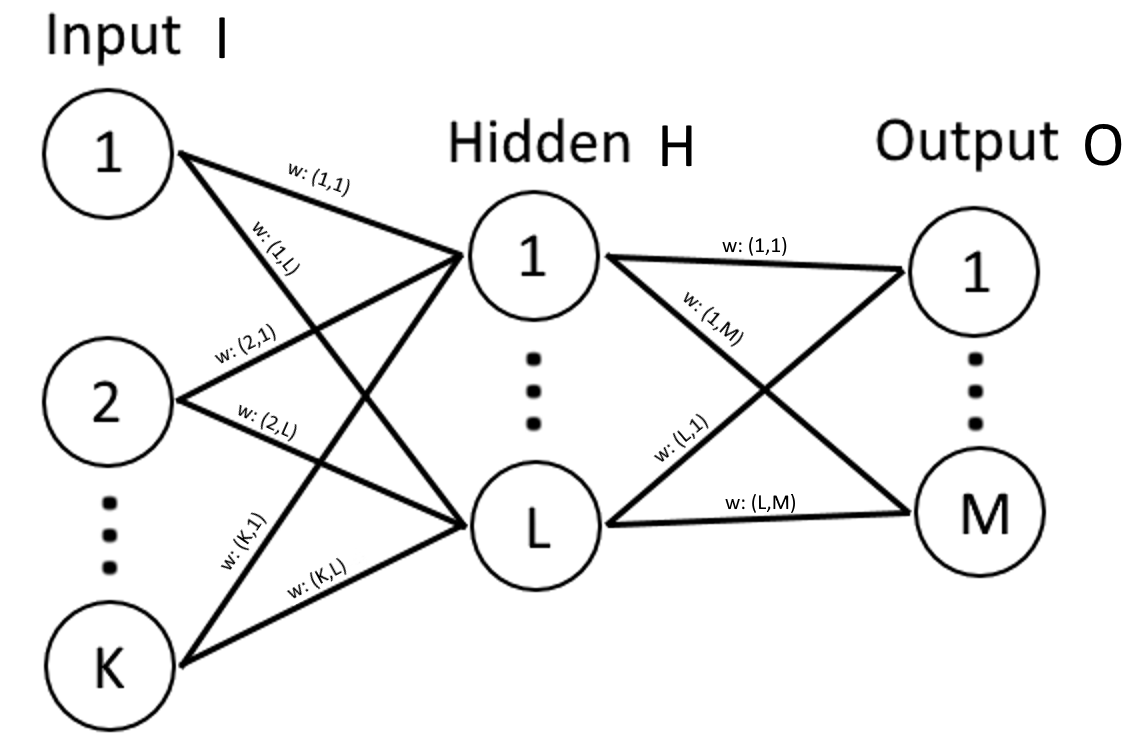
\includegraphics[width=\textwidth]{NeuralNetworkWeights.png}
  \caption{Een neural network met aangegeven weights}
  \label{fig:NeuralNetworkWeights}
\end{figure}

De cost functie is:

$$ C(x) = \frac{1}{2}\sum_{m=1}^{M}(y_{m}-t_{m})^2 $$

Let op dat $\frac{1}{2}$ gewoon wordt toegevoegd om later makkelijker de afgeleide te kunnen bepalen. We moeten ook de afgeleide van de sigmoid functie weten, deze is gelukkig erg simpel, namelijk:

$$ f'(x) = f(u)(1-f(u))) $$

Wat we nu doen is het bepalen van de afgeleide van de cost functie relatief tot de weging van de hidden neuronen naar de output neuronen ($w_{ho}$). Om tot dit resultaat moeten we een aantal keer de ketting regel toepassen:

\begin{align*}
	c'(x) &= (O_{m}-t_{m}) * O' \\
	O' &= O_{m}(1-O_{m}) * H_{l} \\
	c'(x) &= (O_{m}-t_{m}) * O_{m}(1-O_{m})*H_{l}
\end{align*}

Nu we de afgeleide hebben berekend kunnen we de weight een beetje in de goede richting verplaatsen. Hierin staat $\eta$ voor de learning rate (TODO ref).

$$ w_{lm} = w_{lm} - \eta *(O_{m}-t_{m}) * O_{m}(1-O_{m})*H_{l} $$

Om de afgeleide van de cost functie te bepalen relatief tot de weging van de de input neuronen naar de hidden neuronen moeten we nog een aantal keer de ketting regel toepassen, maar uiteindelijk krijgen we de volgende afgeleide:

\begin{align*}
	C'(x) &= \sum_{m=1}^{M}[(O_{m}-t_{m}) * O'] \\
	O' &= O_{m}(1-O_{m}) * H_{l} * H' \\
	H' &= H_{l}(1-H_{l})*I_{k}\\
	C'(x) &= \sum_{m=1}^{M}[(O_{m}-t_{m}) * O_{m}(1-O_{m})*w_{ho}]*H_{l}(1-H_{l})*I_{k}
\end{align*}



De weging $w_{lm}$ wordt dan:

$$ w_{lm} = w_{lm} - \eta *\sum_{m=1}^{M}[(O_{m}-t_{m}) * O_{m}(1-O_{m})*w_{ij}]*H_{l}(1-H_{l})*I_{k} $$

\subsection{Programma}
Bij het opstarten van het programma verschijnt een scherm waarin de beginwaarden van het neural network bepaald kunnen worden en het probleem gekozen kan worden. Als je met de muis op een onderdeel staat verschijnt er meer informatie over het desbetreffende onderdeel.Het wordt erg aangeraden om zelf een paar dingen te proberen en te kijken wat het resultaat is.


\subsection{Resultaten}
TODO

\subsection{Conclusie}
TODO

\end{document}
